

\documentstyle[hyperref,url,pxjahyper,color,subfigure,graphicx,epsf,here,cite,otf,comment,nccmath,mediabb,fancyhdr,12pt]{jarticle}

\hypersetup{
	colorlinks=false, % リンクに色をつけない設定
	bookmarks=true, % 以下ブックマークに関する設定
	bookmarksnumbered=true,
	pdfborder={0 0 0},
	bookmarkstype=toc
}


\graphicspath{{./pic/}}
%%%\documentstyle{jarticle}
\setlength{\textwidth}{16.2cm}%A4
\setlength{\textheight}{23cm}%A4
\setlength{\topmargin}{-1.5cm}
\setlength{\oddsidemargin}{0cm}
\setlength{\evensidemargin}{0cm}
\setlength{\parskip}{1pt}
%\pagestyle{myheadings}
\pagestyle{fancy}
\lhead[名前]{大場 大輔}
\rhead[令和3年4月15日]{令和3年4月19日}
\title{新人ゼミ課題}
\author{大場 大輔}
\date{令和3年4月19日}

\begin{document}
	\maketitle
	\vspace*{20pt}

	
\section*{3.時系列識別}
すでに画像処理やPythonを用いたプログラミングの経験があることと、Brian研究室に配属されたことを考慮して、このコースを選択しました。
なお、本レポートで使用したソースコードはこのページ\footnote{\url{https://github.com/ba-san/assignment2021}}にて確認できます。
まずは、今回のレポートで使用した動的時間伸縮法とk近傍法について簡単に要点を報告します。

\subsection*{動的時間伸縮法について}
動的時間伸縮法(DTW; Dynamic Time Warping)とは、2つの時系列データの距離(類似度)を求める手法であり、具体的には比較するデータの各サンプル同士の距離(今回はユークリッド距離を使用)を総当りで求めて、この2つのデータ間の最短経路を求める手法です。この手法は本研究室の創設者である迫江博昭先生が開発したということで、個人的には非常に驚きました。

\subsection*{k近傍法について}
k近傍法(kNN; k-Nearest Neighbor)とは、データ分類手法の一つであり、あるデータが、その特徴空間上で最近接しているk個の他のデータのクラスの情報をもとに、多数決的にそのデータの所属するクラスを判定する手法です。今回のLevel1からLevel3のケースであれば、test1とtest2の2つのクラスにそれぞれ一つのサンプルしか存在しないため、必然的にk=1のケース、つまり
2つのクラスのDTWの値のうち、小さい方のクラスに属すると考えればよいことがわかります。
%file:///home/daisuke/Downloads/IPSJ-TOD4504005.pdf
%https://qiita.com/hcpmiyuki/items/251586526c5924f09aa3

\newpage

\subsection*{Level1}
この設問においては、まず自分で実際にDTWを実装し、さらにその計算結果が\verb+tslearn+のライブラリで提供されている\verb+dtw+の関数によるものと一致することを確認しました。
その上で下記の通り、各referenceデータに対するクラス1とクラス2との距離を算出し、グラフを描画しました。
結果から、\textbf{test1からtest3はクラス1に、test4からtest6はクラス2に属する}ことがわかりました。

\begin{figure}[h]
\centering
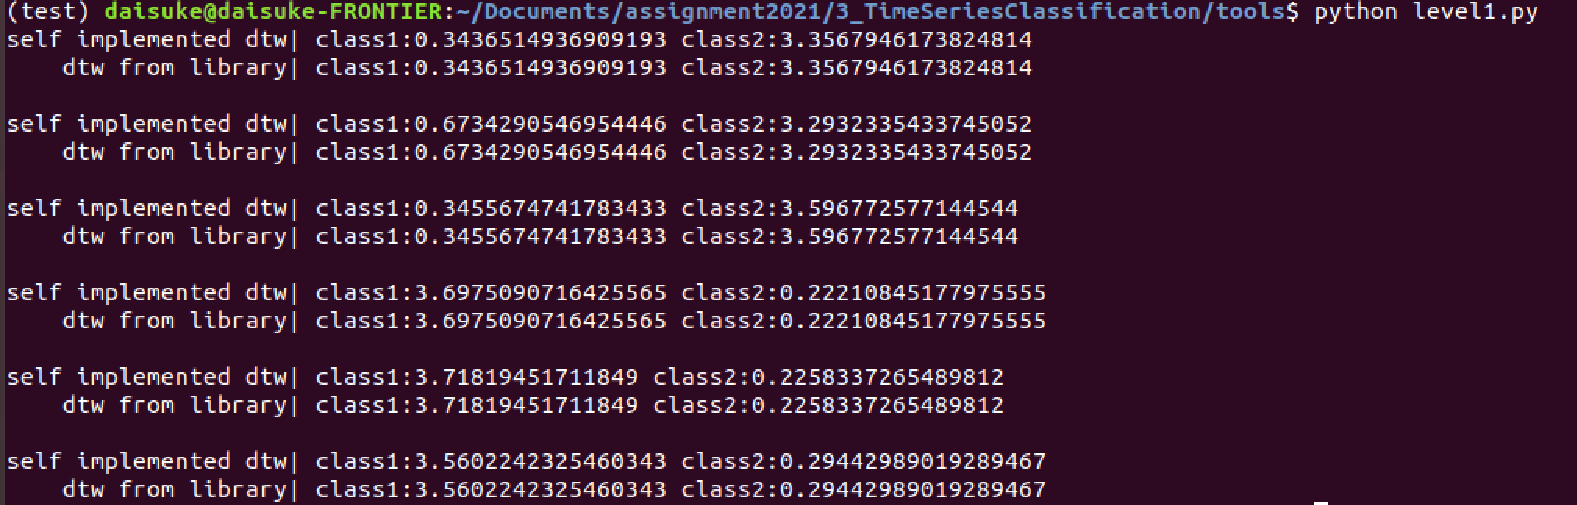
\includegraphics[scale=0.6]{./pic/level1/level1.pdf}
\end{figure}

\begin{figure}[h]
 \begin{minipage}[b]{0.32\linewidth}
  \centering
  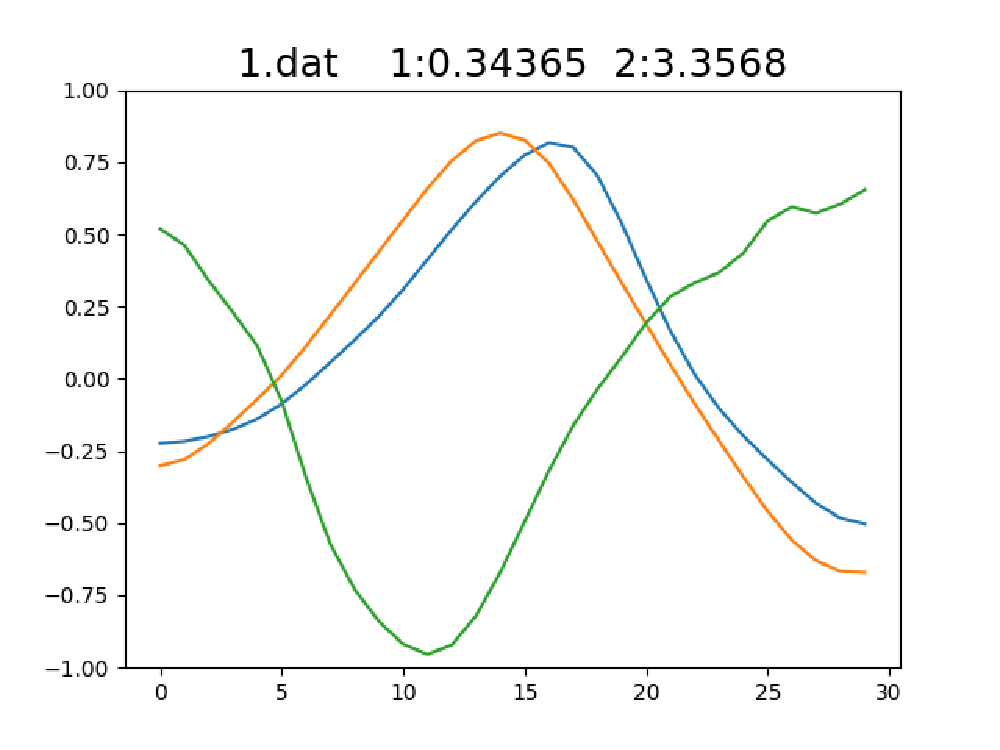
\includegraphics[keepaspectratio, scale=0.3]
  {./pic/level1/1_dat.pdf}
  \label{1dat}
 \end{minipage}
 \begin{minipage}[b]{0.32\linewidth}
  \centering
  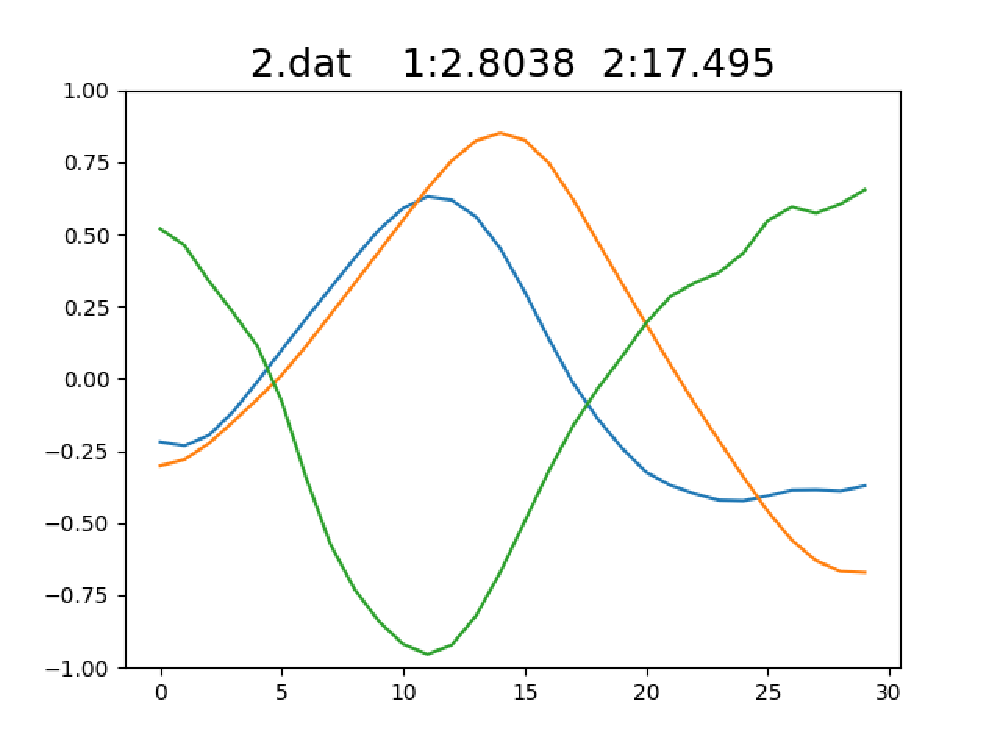
\includegraphics[keepaspectratio, scale=0.3]
  {./pic/level1/2_dat.pdf}
  \label{2dat}
 \end{minipage}
 \begin{minipage}[b]{0.32\linewidth}
  \centering
  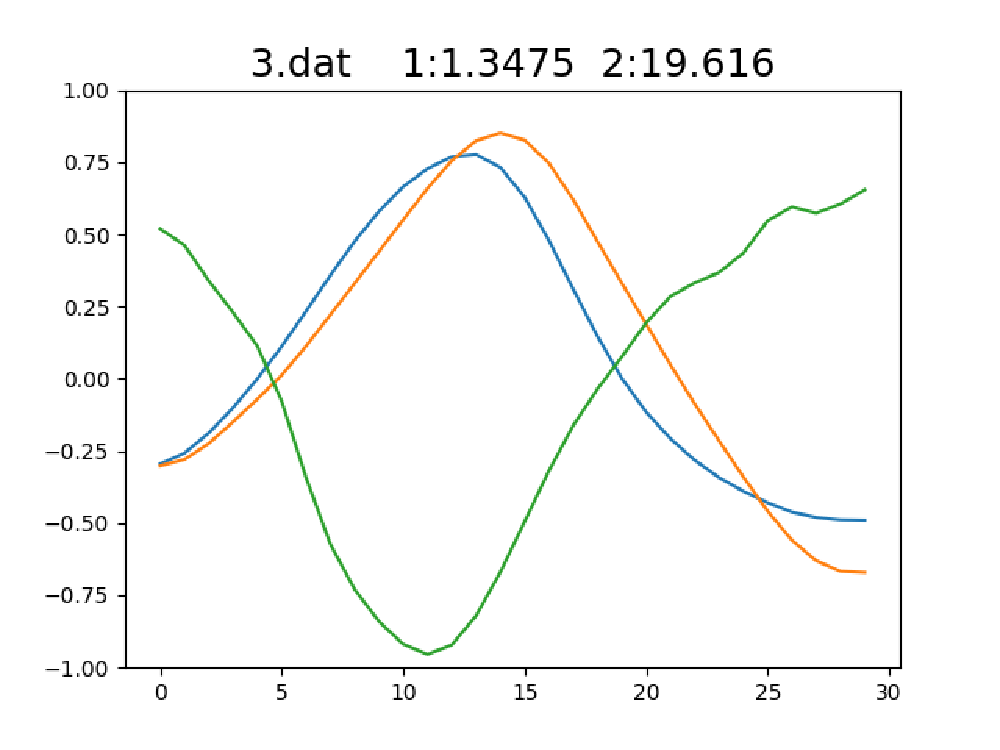
\includegraphics[keepaspectratio, scale=0.3]
  {./pic/level1/3_dat.pdf}
  \label{3dat}
 \end{minipage}\\
 \begin{minipage}[b]{0.32\linewidth}
  \centering
  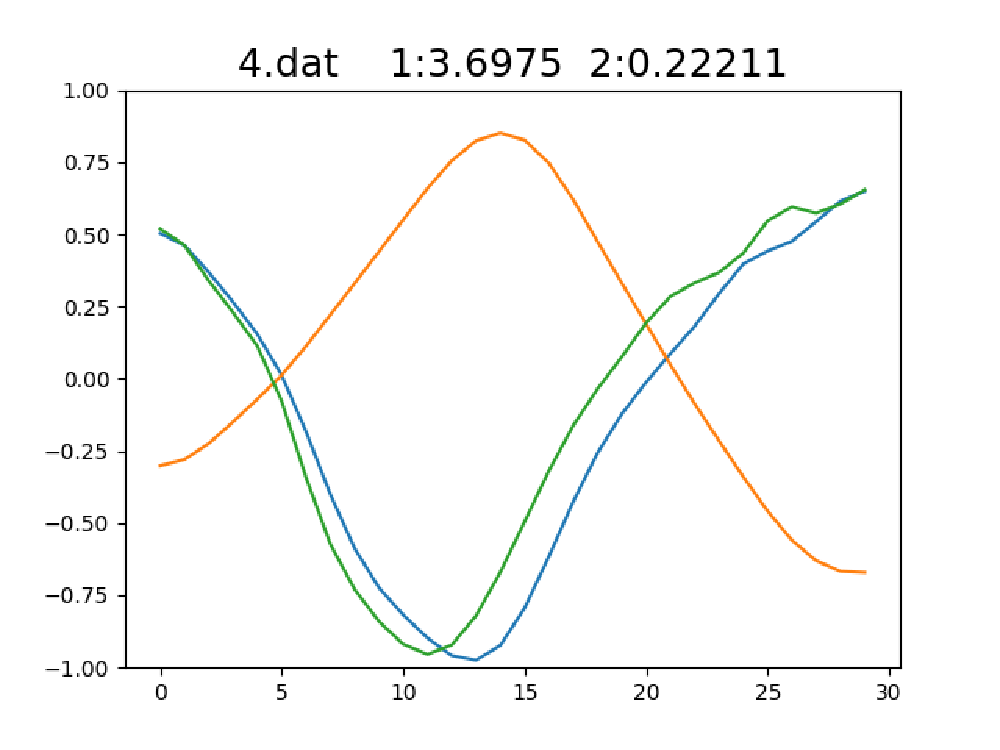
\includegraphics[keepaspectratio, scale=0.3]
  {./pic/level1/4_dat.pdf}
  \label{4dat}
 \end{minipage}
 \begin{minipage}[b]{0.32\linewidth}
  \centering
  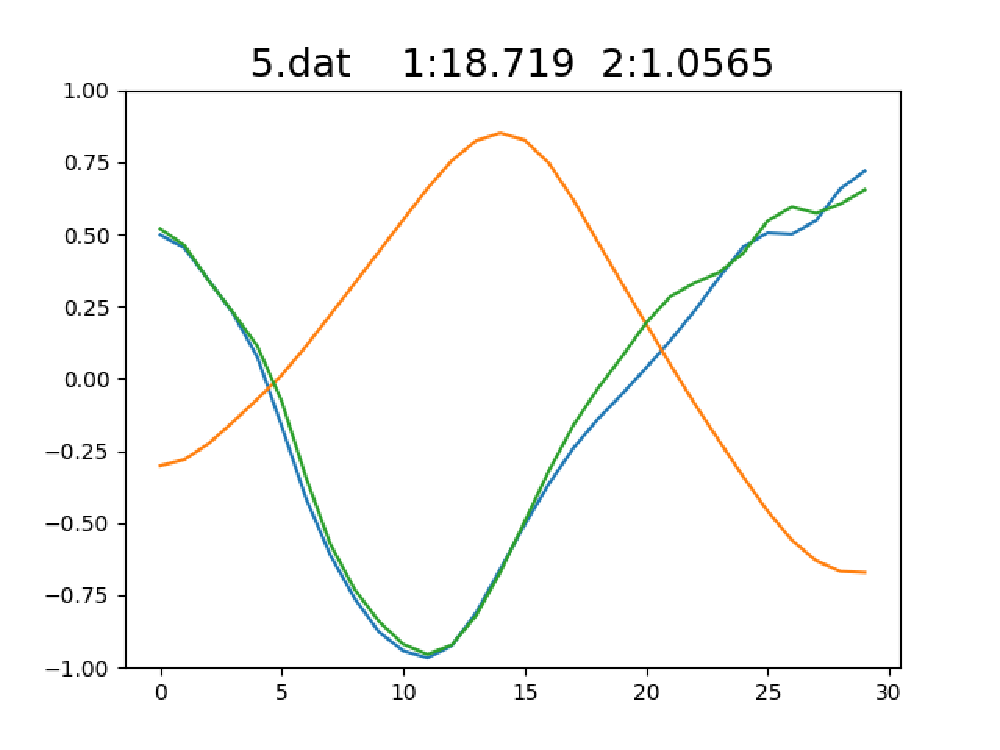
\includegraphics[keepaspectratio, scale=0.3]
  {./pic/level1/5_dat.pdf}
  \label{5dat}
 \end{minipage}
  \begin{minipage}[b]{0.32\linewidth}
  \centering
  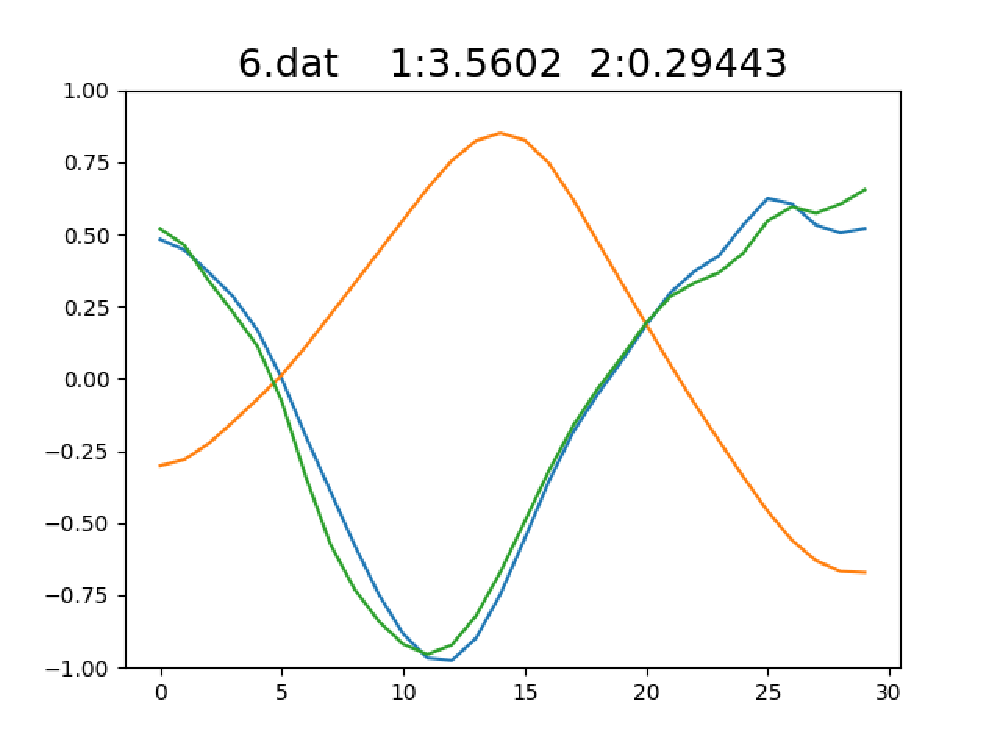
\includegraphics[keepaspectratio, scale=0.3]
  {./pic/level1/6_dat.pdf}
  \label{6dat}
 \end{minipage}
 \caption{各referenceのグラフ。青線が評価対象で、オレンジ線がクラス1、緑線がクラス2を示しています。}\label{reg_poly}
\end{figure}

\newpage

\subsection*{Level2}
この設問はLevel1で作成した自作\verb+dtw+のコードを3次元ベクトルに対応できるように拡張したことで解決しました。
結果から、\textbf{test1,test3,test6はクラス1に、test2,test4,test5はクラス2に属する}ことがわかりました。

\begin{figure}[h]
 \begin{minipage}[b]{0.32\linewidth}
  \centering
  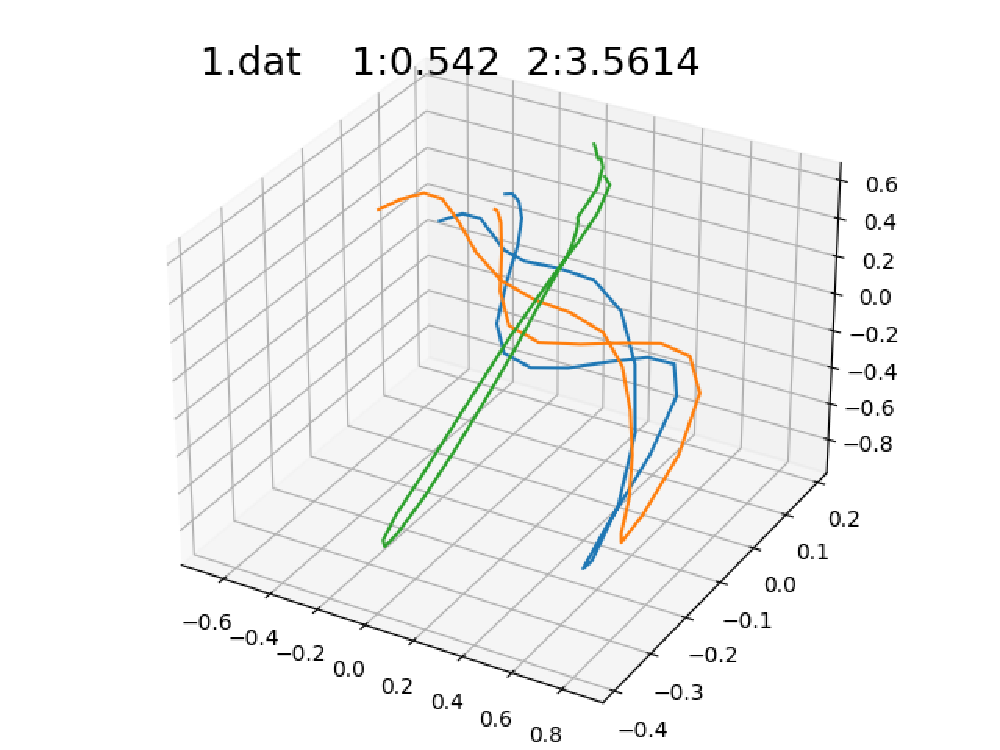
\includegraphics[keepaspectratio, scale=0.3]
  {./pic/level2/1_dat.pdf}
  \label{1dat}
 \end{minipage}
 \begin{minipage}[b]{0.32\linewidth}
  \centering
  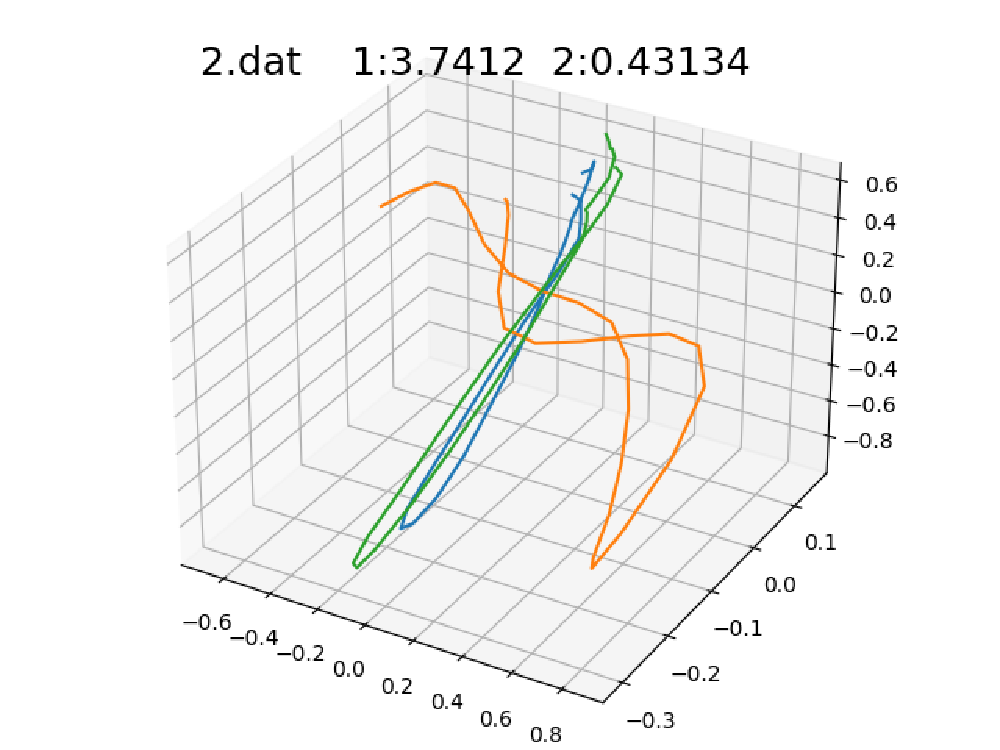
\includegraphics[keepaspectratio, scale=0.3]
  {./pic/level2/2_dat.pdf}
  \label{2dat}
 \end{minipage}
 \begin{minipage}[b]{0.32\linewidth}
  \centering
  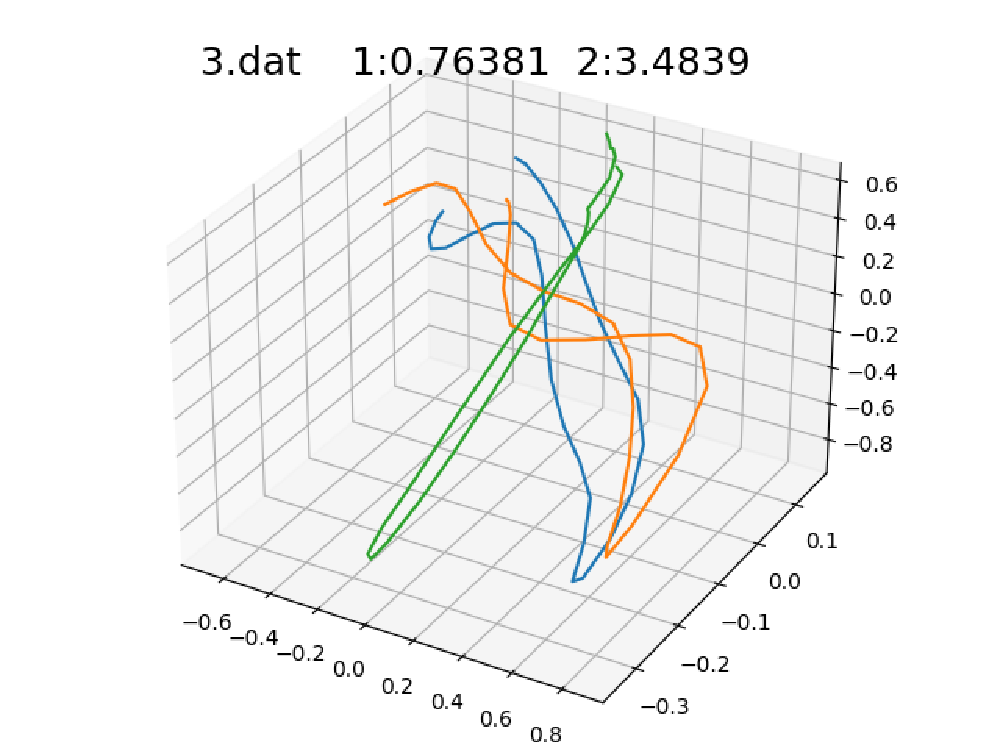
\includegraphics[keepaspectratio, scale=0.3]
  {./pic/level2/3_dat.pdf}
  \label{3dat}
 \end{minipage}\\
 \begin{minipage}[b]{0.32\linewidth}
  \centering
  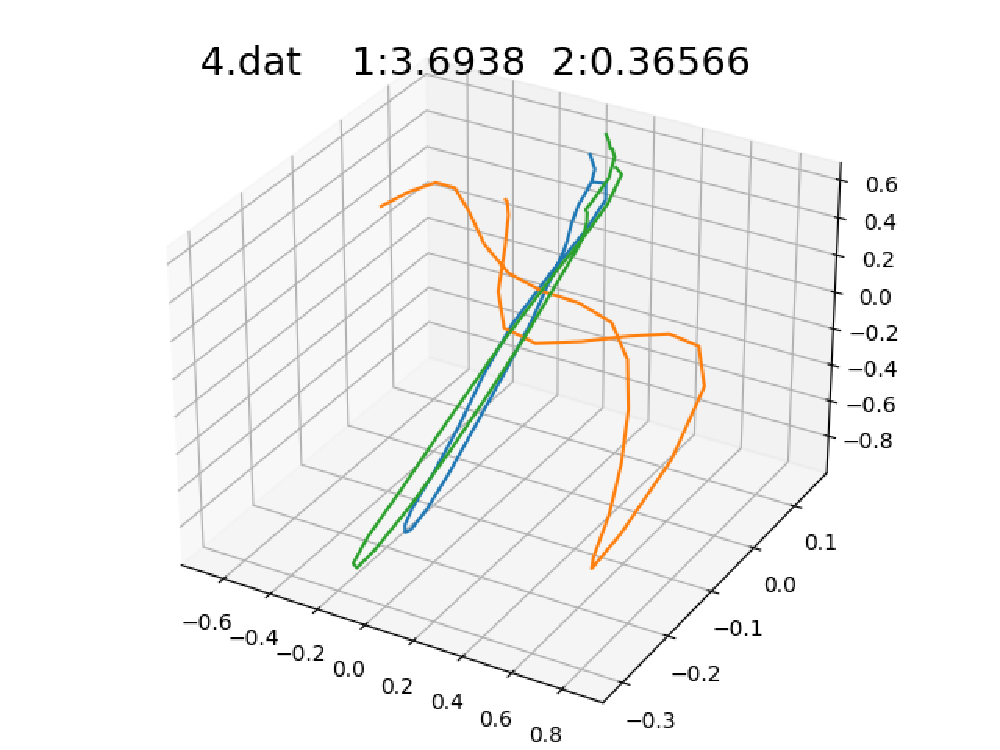
\includegraphics[keepaspectratio, scale=0.3]
  {./pic/level2/4_dat.pdf}
  \label{4dat}
 \end{minipage}
 \begin{minipage}[b]{0.32\linewidth}
  \centering
  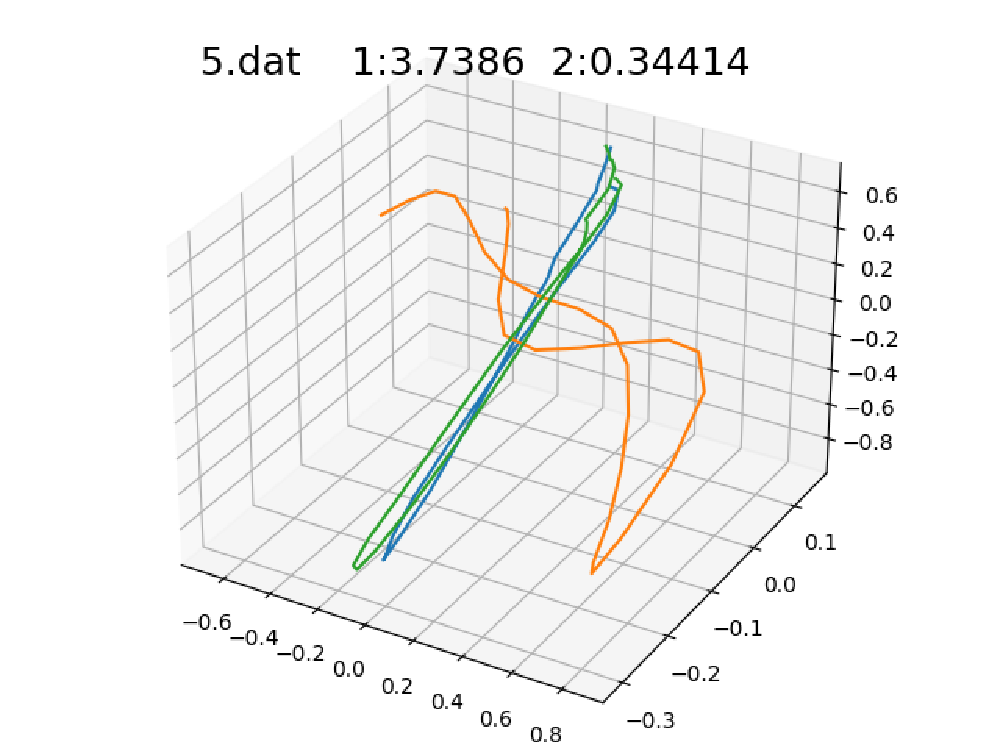
\includegraphics[keepaspectratio, scale=0.3]
  {./pic/level2/5_dat.pdf}
  \label{5dat}
 \end{minipage}
  \begin{minipage}[b]{0.32\linewidth}
  \centering
  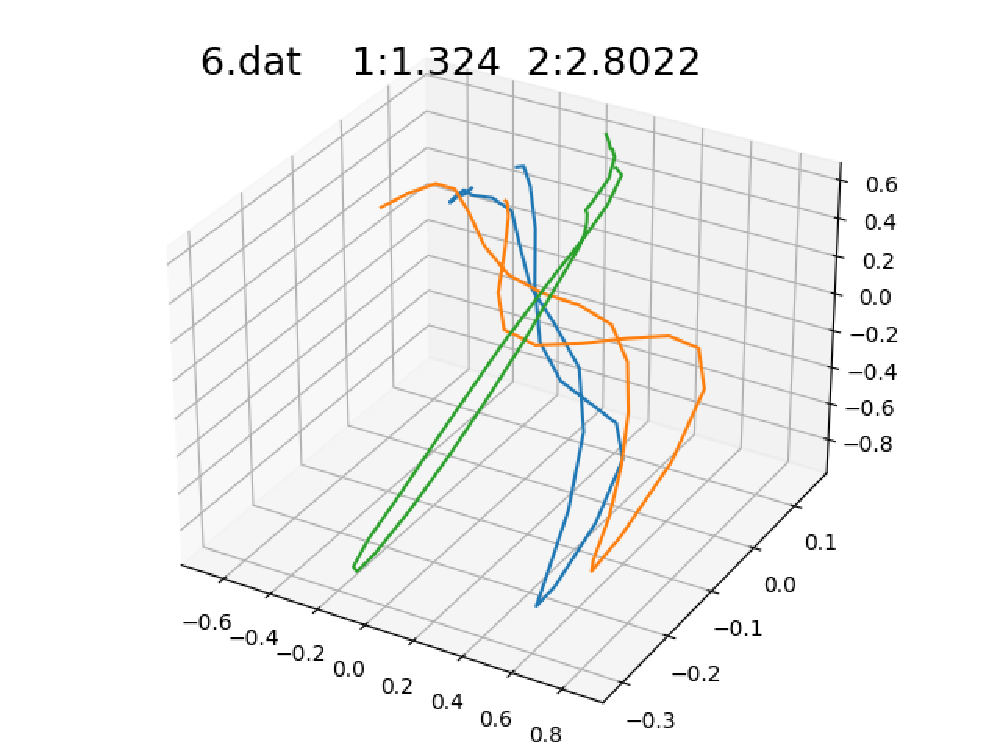
\includegraphics[keepaspectratio, scale=0.3]
  {./pic/level2/6_dat.pdf}
  \label{6dat}
 \end{minipage}
 \caption{各referenceのグラフ。青線が評価対象で、オレンジ線がクラス1、緑線がクラス2を示しています。}\label{reg_poly}
\end{figure}

\subsection*{Level3}
この設問はLevel2で使用した自作\verb+dtw+のコードにおいて、累積行列を時系列長の大きい方に合わせた正方行列にすることで、可変長でも対応できるように改変しました。
結果から、\textbf{test1,test3,test6はクラス1に、test2,test4,test5はクラス2に属する}ことがわかりました。

なお、test3とtest5の結果はLevel2のときと異なっています。これはLevel3のデータがLevel2のものと、test3とtest5に限っては対応づいていないことが推測されます。(例えばLevel3のtest3のデータはLevel2のtest3のデータではなく、test5をベースに改変されたものだとグラフの形状から推測されます。逆も同じです。)

\begin{figure}[h]
 \begin{minipage}[b]{0.32\linewidth}
  \centering
  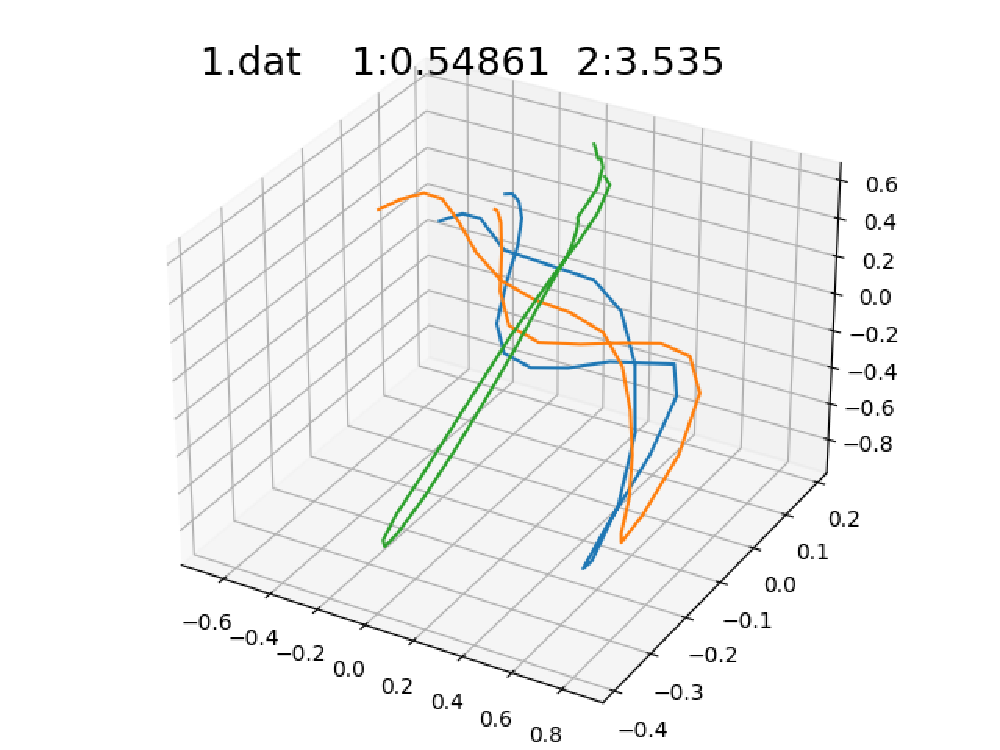
\includegraphics[keepaspectratio, scale=0.3]
  {./pic/level3/1_dat_l3.pdf}
  \label{1dat}
 \end{minipage}
 \begin{minipage}[b]{0.32\linewidth}
  \centering
  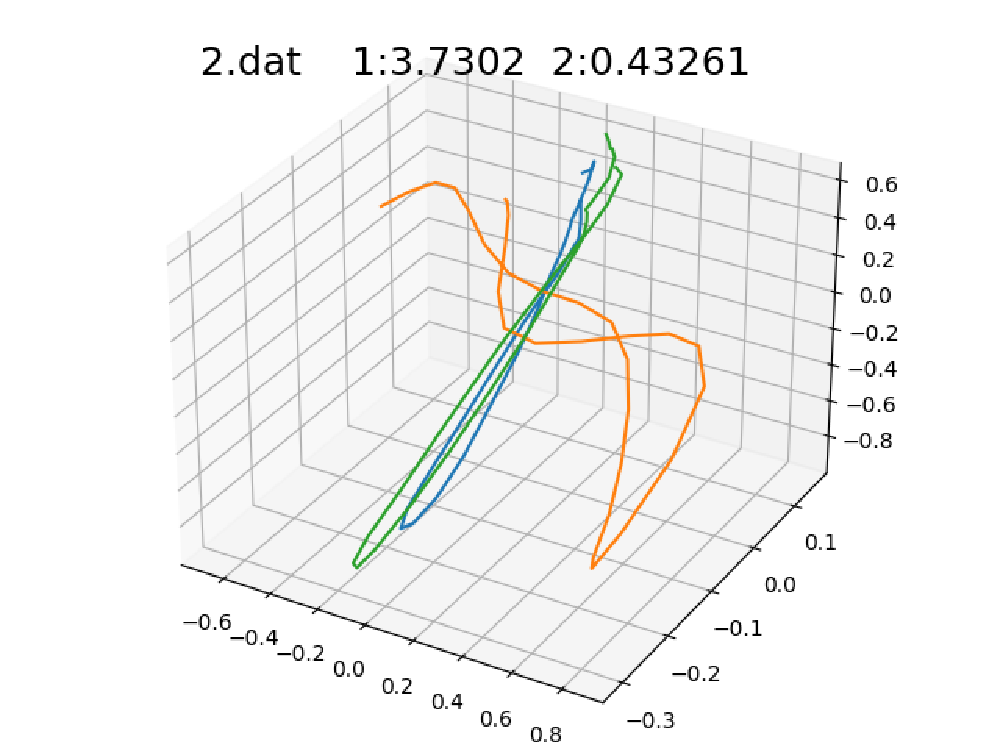
\includegraphics[keepaspectratio, scale=0.3]
  {./pic/level3/2_dat_l3.pdf}
  \label{2dat}
 \end{minipage}
 \begin{minipage}[b]{0.32\linewidth}
  \centering
  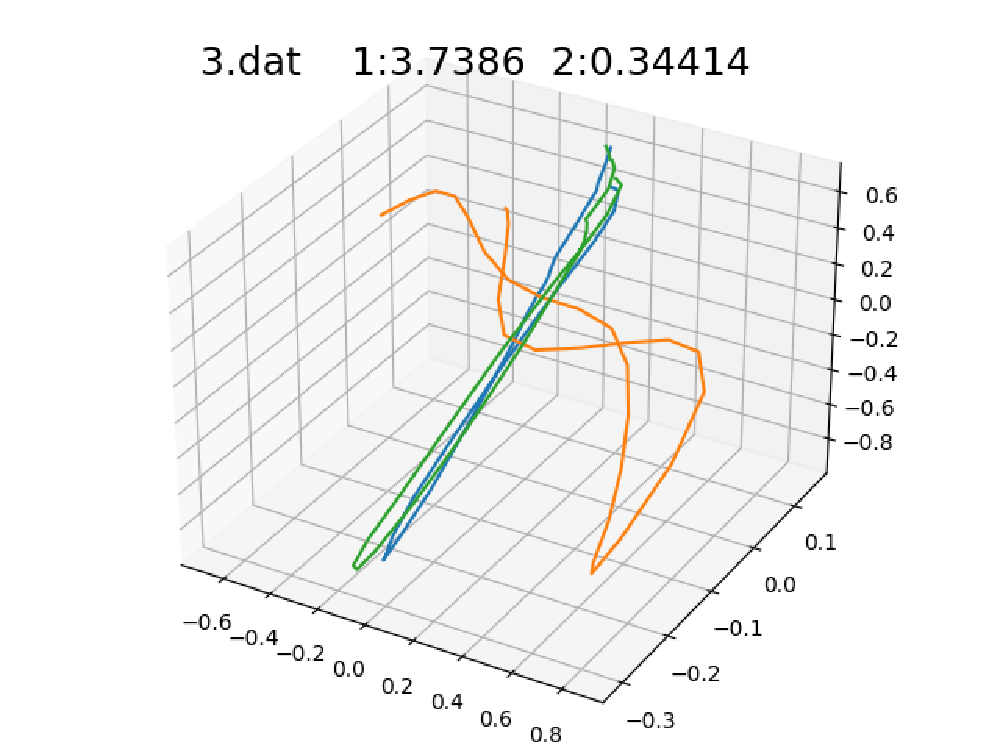
\includegraphics[keepaspectratio, scale=0.3]
  {./pic/level3/3_dat_l3.pdf}
  \label{3dat}
 \end{minipage}\\
 \begin{minipage}[b]{0.32\linewidth}
  \centering
  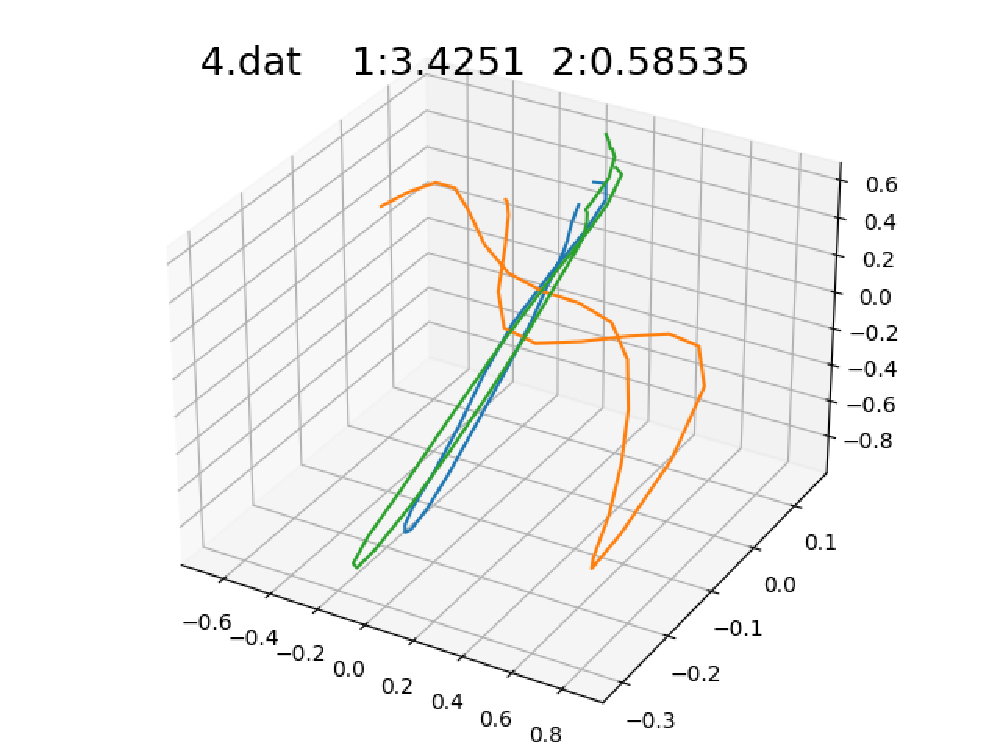
\includegraphics[keepaspectratio, scale=0.3]
  {./pic/level3/4_dat_l3.pdf}
  \label{4dat}
 \end{minipage}
 \begin{minipage}[b]{0.32\linewidth}
  \centering
  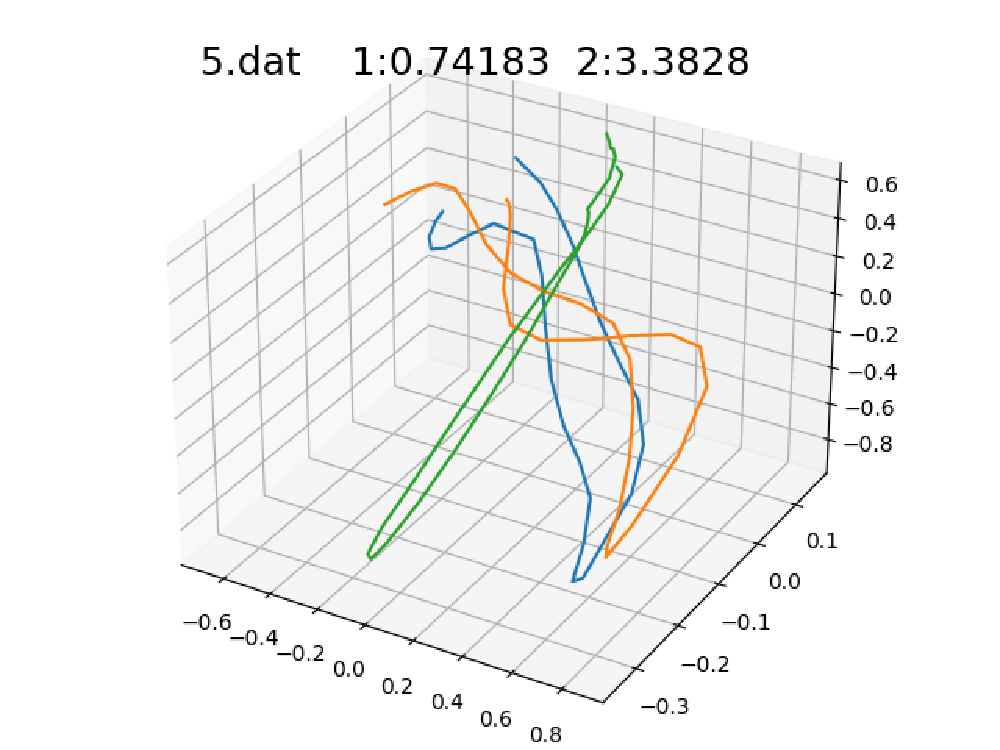
\includegraphics[keepaspectratio, scale=0.3]
  {./pic/level3/5_dat_l3.pdf}
  \label{5dat}
 \end{minipage}
  \begin{minipage}[b]{0.32\linewidth}
  \centering
  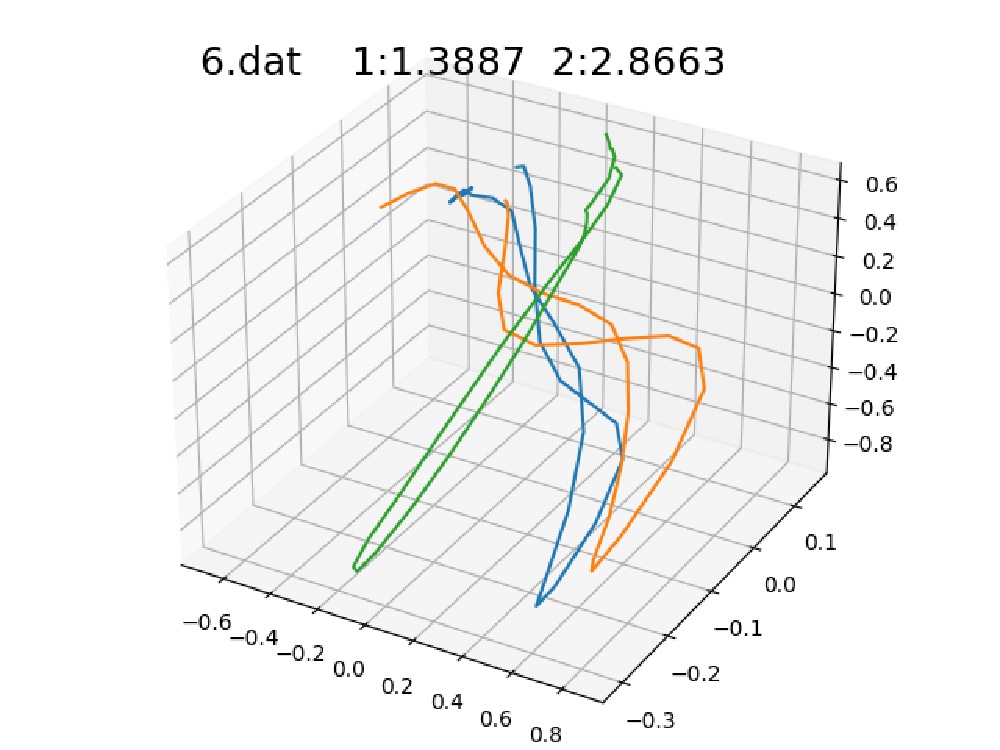
\includegraphics[keepaspectratio, scale=0.3]
  {./pic/level3/6_dat_l3.pdf}
  \label{6dat}
 \end{minipage}
 \caption{各referenceのグラフ。青線が評価対象で、オレンジ線がクラス1、緑線がクラス2を示しています。}\label{reg_poly}
\end{figure}

\newpage

\subsection*{Level4}
まずは、これまでと同様にして

この設問は、Brian先生の新人ゼミの内容からTCN(Temporal Co)が訓練時間が短く、高い精度を出すと紹介されていたので、この手法を用いて推定を行いました。
%主成分分析使えれば次元削減は可能だが...
	
	
	
\end{document}
